\newpage
\section{Określenie wymagań szczegółowych}		%2
%Dokładne określenie wymagań aplikacji (cel, zakres, dane wejściowe) – np. opisać przyciski, czujniki, wygląd layoutu, wyświetlenie okienek. Opisać zachowanie aplikacji – co po kliknięciu, zdarzenia automatyczne. Opisać możliwość dalszego rozwoju oprogramowania. Opisać zachowania aplikacji w niepożądanych sytuacjach.

\hspace{0.60cm}Firma nie związana z technologia pragnie aby stworzyć aplikację mobilną do testowania czujników, która byłaby  zachowana w sposób minimalistyczny i intuicyjny. Przejrzysta i prosta budowa menu, która miałaby na celu usprawnić szukanie odpowiednich komponentów. Firma posiada również logo, które powinno zawierać się w projekcie, jak i niebieskie akcenty (np. przyciski) - który jest przewodnim kolorem firmy. \newline

Jednym z kluczowych zadań jest stworzenie aplikacji w sposób jak najbardziej przejrzysty, do tego celu użyjemy ikonek, które w prosty i szybki sposób nakierują nas na odpowiedni komponent. Przykładem może być latarka; chcąc przetestować jej działanie wystarczy wybrać ikonkę która będzie przedstawiała latarkę. Po jej naciśnięciu zostaniemy przekierowani do strony z testem, który będzie posiadał dwa przyciski jeden to zielony włącznik oraz czerwony wyłącznik. Ponadto będziemy starać się aby wyniki testów były stopniowo zapisywane w pliku wyjściowym. Jako wykonawcy aplikacji chcielibyśmy wdrożyć do projektu przyciski które znajdowałyby się przy każdym teście i informowałyby o tym ,że: "test przebiegł pomyślnie" lub "test nie powiódł się". W zależnie od tego który przycisk naciśniemy to w taki sposób uzupełni się plik wyjściowy z podsumowaniem testu. Zapewniamy również zawarcie logotypu i motywu niebieskiego aplikacji, i sprawimy by layout w całości był jak najbardziej intuicyjny i zachowany w minimalistyczny sposób (brak jaskrawych kolorów, duże przejrzyste przyciski, okienka pop-up z wiadomościami o przebiegu testu). Postaramy się aby komponenty testujące takie jak: latarka, test dźwięku, czujnik światła, tryb nocny i tym podobne; będą poprawnie spełniać swoje zadanie. Aplikacja zostanie napisana w programie Android Studio, natomiast język którym będziemy się posługiwać to: Java. \newline

Tak jak już wspomnieliśmy powyżej postaramy się by każdy z czujników działał w należyty sposób; to znaczy by latarka poprzez kliknięcie przycisków włączała się i wyłączała. Test dźwięku pozwoli nam poprzez kliknięcie przycisku usłyszeć z głośników wydobywającą się melodię; tryb nocny, który jest bardzo przydatną funkcją w telefonie szczególnie wieczorami gdy korzystamy z urządzeń mobilnych, zmieni kolorystykę z jasnej na ciemną. Przez tą funkcję jaka jest tryb ciemny nasze oczy nie są narażane na tak mocne światło, co sprawia, że czujemy większy komfort w użytkowaniu telefonów komórkowych. Niektóre osoby preferują korzystanie z trybu nocnego nawet podczas dnia a nie tylko nocą. Kolejny czujnik jakim będzie GPS pozwoli nam w szybki sposób określić położenie w którym się znajdujemy. Test Wifi umożliwi spawdzenie połączenia z siecią, natomiast test mikrofonu sprawdzi się w sytuacji gdy na przykład pojawi się problem podczas rozmów telefonicznych. Test aparatu pozwoli wykonać zdjęcie oraz przetestować jakość wykonanego zdjęcia.  \newline
Pragnieniem firmy, która zleciła nam wykonanie aplikacji, jest stworzenie panelu logowania, dzięki któremu pracownicy wraz z klientami będą mogli logować się do aplikacji. Naszym zdaniem nie ma konieczności do tworzenia odrębnego panelu do logowania, ponieważ aplikacja wykonuje tylko testy czujników i nie przechowuję poufnych danych. Co więcej w sytuacji gdy kilkaset osób postanowi wejść w aplikację i zalogować się na nią, może dojść do przeciążenia i zawieszenia się strony, co wiążę się z tym, że nabywcy aplikacji będą musieli poczekać dłuższą chwilę aby logowanie się powiodło. Uważamy, że w dużych firmach mogłoby to spowolnić pracę pracowników, a czas pracy odgrywa bardzo ważną rolę.\newline

Rozpoczęliśmy pracę przy tworzeniu wstępnego layout strony głównej (rysunek 2.1) i na ten moment prezentuję się ona następująco: \newline 
 \begin{figure}[!hbt]
	\begin{center}
		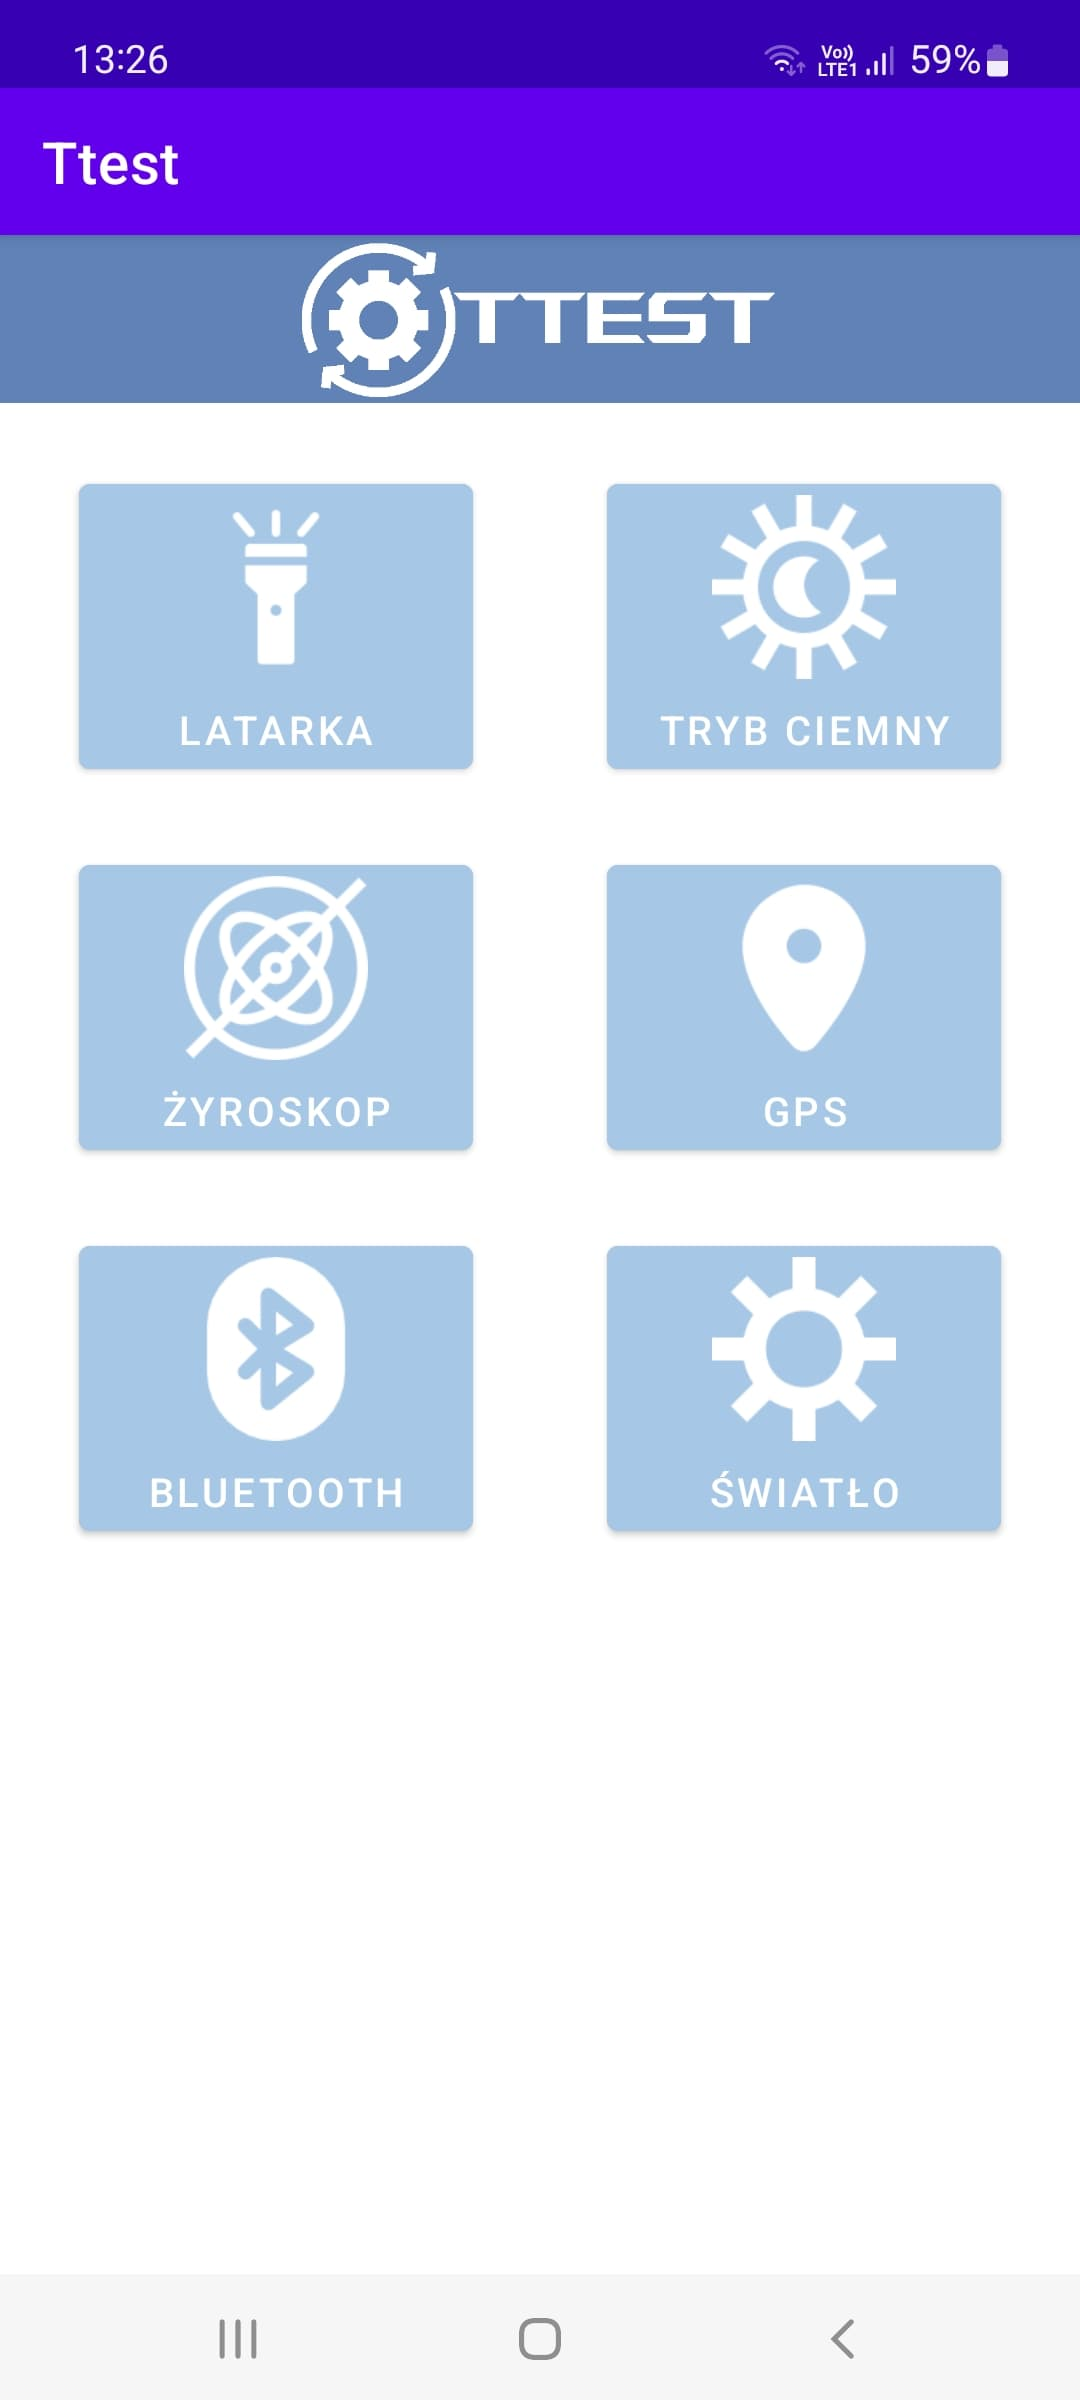
\includegraphics[angle=360, width=0.31\textwidth]{rys/menu.jpg}
		\caption{Wstępne menu}
		\label{rys:Menu}
	\end{center}
\end{figure}
\newpage
Na tą chwilę udało nam się stworzyć menu z sześcioma przyciskami, które prezentują poszczególne czujniki. Aktualnie przyciski nie przekierowują jeszcze na stronę testów lecz tym zajmiemy się w kolejnym etapie naszej pracy. Co więcej na górze ekranu dokładniej w jego centrum umieszczone zostało logo firmy, które dostaliśmy w zleceniu. Kolorystyka jest utrzymana w błękicie oraz bieli. 

